\documentclass{article}

\usepackage[final]{neurips_2019}

\usepackage[utf8]{inputenc}
\usepackage[T1]{fontenc}
\usepackage{url}
\usepackage{booktabs}
\usepackage{amsfonts}
\usepackage{amssymb}
\usepackage{nicefrac}
\usepackage{microtype}
\usepackage{graphicx}
\usepackage{verbatim}
\usepackage{xcolor}
\usepackage{lipsum}
\usepackage{xcolor}
\usepackage[colorlinks = true,
            linkcolor = blue,
            urlcolor  = blue,
            citecolor = blue,
            anchorcolor = blue]{hyperref}
\newcommand{\note}[1]{\textcolor{blue}{{#1}}}
\newcommand{\abs}[1]{\left| #1\right|}
\usepackage{amsmath}

\title{
  Translating Natural Language to Bash Commands using Deep Neural Networks \\
  \vspace{1em}
  \small{\normalfont Stanford CS224N Custom Project}
}

\author{
 Daniel Jenson \\
  Department of Management Science \& Engineering \\
  Stanford University \\
  \texttt{djenson@stanford.edu} \\
  % Examples of more authors
  \And
  Yingxiao Liu \\
  Department of Civil and Environmental Engineering \\
  Stanford University \\
  \texttt{liuyx@stanford.edu} \\
}

\begin{document}

\maketitle

\begin{abstract}
The objective of this project is to generate bash commands from natural language using a deep neural network. We used the NLC2CMD dataset, templatized the data, and experimented with several models, including GPT-2, BART, and T5, as well as different tokenization schemes and postprocessing methods to improve model performance on the NLC2CMD dataset. We found that although BART and GPT-2 models got the lowest cross-entropy loss, T5 achieved the highest score measured with the defined metric and beat the baseline model. (maybe add something about the source of error or the future work)
\end{abstract}


\section{Key Information to include}
\begin{itemize}
	\item TA mentor: Ethan A. Chi
	\item External collaborators: No
	\item External mentor: No
	\item Sharing project: No
\end{itemize}

% {\color{red} This template does not contain the full instruction set for this assignment; please refer back to the milestone instructions PDF.}

\section{Introduction}
ash, the Unix command language, has long been used to interact with computers universally, expressively and efficiently.  However, due to the existence of numerous bash utilities (e.g. ``find'', ``cd'', ``mkdir'') and flags (e.g. ``-f'', ``-r'' ), novitiates often find the terminal interface perplexing and are quickly overwhelmed by the syntax of Bash commands. Even experienced engineers frequently consult man-pages, online documentation, and online forms like Stack Overflow to learn about the particulars of various commands. This project aims to ease those burdens on new and experienced users alike, and develop tools to generate Bash commands from natural language. We want to provide a NLI (Natural Language Interface) enable people to interact with computers through natural languages, and make the programming resources more accessible to the public.

However, translating natural language into bash can be challenging: different users have different ways to express logical statement in natural language; a single task may involve pipelines of different utilities, and the order of these utilities matters; one utility can be associated with multiple flags, and different flags can be switched; there are a lot of identifiers like specific paths or file names in bash commands, and we need a way to generalize our model predictions; and finally, the bash commands must be perfectly correct before they can be executed in terminals. Although it is impossible to solve all these problems, we tried to tackle some of them.

In this work, we used the data from the NeurIPS 2020 NLC2CMD Challenge, and experimented with several transformer models, including GPT-2, BART, and T5, as well as different tokenization and postprocessing schemes to generate bash commands from natural language. We evaluated the model performance from both the training loss and a specific metric measuring how similar two Bash commands are, and compared our models with the baseline model provided in the competition. 


\section{Related Work}
Code generation is a variant of semantic parsing, and a number of research works have been published in this area. One of the earliest and most successful studies was conducted to translate the natural language to SQL query, and Zhong et al. (2017) \cite{zhong2017seq2sql} proposed a deep augmented pointer network and achieved an execution accuracy of 60\% when combined with reinforcement learning. However, it must be taken into consideration that SQL is more like a domain specific language with a much simpler syntax.

For high level programming language generation, there are recent attempts to translate well structured natural language input into Java or Python.  Ling et al. (2016) \cite{ling2016latent} proposed a generative mode with a multiple pointer network to generate code from texts in Trading Card Games, and such input language is rather formal. A more robust syntax-based model has been developed by Yin and Neubig (2017) \cite{yin2017syntactic} and tested on the same dataset, but the result was only found to be equally good. Rahit et al. (2019) \cite{rahit2019machine} used recurrent neural network (RNN) and long-short term memory (LSTM) to build their model and reported an accuracy as high as 74\% when the input was prepared in a format closer to pseudo code with keywords such as “define” and “if-else”. 

In the specific domain of Bash command generation, Lin et al. (2018) \cite{lin2018nl2bash} modified the seq2seq model by adding gated recurrent units (GRU) and RNN cells, and introducing a copying mechanism. The model was evaluated manually by people, rather than by an objective metric, and the accuracy was reported to be 0.29. This again confirmed the difficulty of the natural language to bash translation.

\color{red}
\section{Approach}
\color{black}
The NLC2CMD Challenge was held once by NeurIPS in 2020. The provided dataset
consists of 10,000 parallel translations as a JSON. The goal for competitors
was to generate templated commands from natural language commands that could be
used to guide bash users. Most competitors used GPT2 as their base model. This
paper also uses GPT2 but also surveys two additional models, BART and T5,
version 1.1.
\par
The general approach consisted of two principle methods: (1) text generation
and (2) translation. First, it is important to note that Bash is not a
context-free grammar. It admits of very little recursion and, while most
binaries are POSIX compliant, their interfaces are non-standardized. Flags
often carry different semantic meaning and imply different tasks when employed
by different binaries. Moreover, flags often override, modify, or cancel the
intent of other flags in the same command, introducing complex dependencies.
These dependencies can also shift as the order of the flags and their arguments
are permuted. In sum, the meaning of a flag is almost entirely provided by the
invoking binary and its location in the sequence of arguments. This introduces
difficulties in fine-tuning embeddings, since training may attempt to encode
vastly different meanings in the same embedding. This is particularly
challenging given sparse datasets. Given sufficient training data, it is likely
that that the models may eventually learn correct contextual meaning when
employed by different binaries, but we found 10,000 rows insufficient for the
task. This line of thinking inspired our first approach, text generation using
GPT2.
\par
While at first this task appears to be a straightforward translation task,
after considering bash more closely, one can see that it does not admit of many
properties or structures of natural language. Accordingly, we thought that
rather than trying to properly translate natural language into bash, we could
train a model to hallucinate bash ``stories'' given natural language. The
high-level idea here is that we fine-tune a GPT2 model, showing it complete
stories that consist of both a natural language portion and a bash portion with
some added special tokens. When training, GPT2 learns common storylines,
and when testing, we feed the trained model only the first half of the
story, i.e. the natural language portion, and ask it to complete the story,
hoping that it will generate bash commands as the most likely story completion.
In many respects, this idea performs quite well; however, a significant issue
with this approach is constraining responses from GPT2. How long should the
story be? When does the real content of the ``bash story'' start and end? What
happens when GPT2 has multiple endings? These questions are detailed in the
error analysis section.
\par
The second approach we used was a more traditional seq2seq language modeling
approach. Pre-trained models for BART and T5 are easily fine-tuned for
translation tasks. While many natural language modeling tasks admit of a fair
amount of transfer learning because natural languages share some abstract
semantic structures, bash does not benefit from this nearly as much. As a
non-natural, non-context-free grammar language, modeling it can be difficult,
and our BART model, in particular, struggled with this.

\section{Experiments}
In this section, we will show the our experimental details and discuss on the results.

\subsection{Data}
The dataset we used is from the ``\href{https://nlc2cmd.us-east.mybluemix.net/}{The NLC2CMD Competition},'' consisting of 10,000 parallel translations of English (named as the ``invocation'') and bash command (named as the ``cmd''), and one example is shown as follows:

\begin{verbatim}
invocation: Assign permissions 755 to directories in the current directory tree
cmd: find . -type d -print0 | xargs -0 chmod 755
\end{verbatim}

Instead of a single task, most of the invocations involve a sequence of different tasks, and consequently the bash commands are usually in the form of long pipelines. In addition, since the bash commands contain identifiers, such as directory paths, file names, and permissions, a templatization scheme has been used by casting the shell commands into the corresponding abstract syntax trees (AST), replacing the identifiers and then casting the AST back to commands. The guide can be found \href{https://github.com/IBM/clai/tree/nlc2cmd}{here}. After this step, the command we saw in the previous example were templatized into
\begin{verbatim}
cmd: find Path -type d -print0 | xargs -0 -I chmod Permission
\end{verbatim}
for easier generalization during training.

The invocations and templatized commands can be fed directly into the sequence to sequence models (i.e. BART and T5) as inputs and labels for training. However, for the causal language model GPT-2, additional preprocessing much be performed because such model can only generate code token by token and there is no label at all. We introduced special tokens to separate the invocations and commands, and assemble them in the form of 

\begin{verbatim}
<bos_token> <source_token> <invocation> <target_token>

                                              <templatized cmd> <eos_token> 
\end{verbatim}

The dataset was split into the training and test sets with a ratio of 0.98 : 0.02.

\subsection{Evaluation method}
The standard cross-entropy loss function was used to trained the models. But a more robust metric measuring the execution accuracy of the model predictions must be used, and we used the metric defined by the competition as
\begin{align*}
	S(p) & =\sum_{i\in[1,T]}\frac{1}{T}\times\left(
	\mathbb{I}[U(c)_i=U(C)i]\times\frac{1}{2}\left(
		1+\frac{1}{N}\left(X\right)\right) -\mathbb{I}[U(c)_i\ne U(C)_i]
	\right)
\end{align*}
where $U(x)$ is a sequence of bash utilities in a command $x$, $c$ is the
predicted bash command and $C$ is the ground truth bash command. 
Apart measuring whether the utilities in the two commands match, an additional variable $X$ has been introduced to measure whether the flags associated with each utility match or not, as 
\begin{equation*}
X = 2\times
	|F(U(c)_i)\cap F(U(C)_i)| - |F(U(c)_i)\cup F(U(C)_i)|
\end{equation*}
where $F(x)$ refers to
the set of bash flags in a command $x$. $T$ is the maximum length between
$U(c)$ and $U(C)$ while $N$ is the maximum size between $F(c)$ and $F(C)$. Since the order of flags does not matter, set operations have been used here.

This is a very strict metric penalizing for both incorrect and extra bash utilities and flags. The return value of the metric is between -1.0 and 1.0, and only a command which produces exactly the same execution result as the ground truth one can get a score of 1.0.

\subsection{Baseline model}
We used the black-box GPT-3 model provided by the competition as the baseline model. This model was reported to achieve a score of -0.13 measuring with the aforementioned metric, and we compared our model performance with this number.

\color{red}
\subsection{Experimental details}
\color{black}
For this task, we tested 3 models: HuggingFace's
\href{https://huggingface.co/gpt2}{GPT2}\cite{gpt2},
\href{https://huggingface.co/facebook/bart-large}{Facebook's BART
	Large}\cite{bart}, and \href{https://huggingface.co/google/t5-v1_1-base}{Google's T5 v1.1
	base}. GPT2 was a causal model, predicting text from context, while the other
two were traditional seq2seq models. Each was trained for 5, 10, and 25
epochs. Batch size was limited to 10 examples, except for T5, which had to be
reduced to 5. For training, we used the AdamW optimizer with weight decay
regularization. The learning rate was linear with a warmup of 100 steps. The
dataset was split into 98\% training and 2\% test sets. Given that the
dataset was approximately 10,000 parallel translations, the test set was
slightly over 200 examples. Training time for GPT, BART, and T5v1.1 was
approximately 1, 1.5, and 1.25 hours, respectively, on an Azure NC6 instance
with a Tesla V100 PCIe 16GB GPU. We attemtped training the original T5 large
model, but even with 5 examples per batch, we got out of memory errors, and
it took approximately 6 hours to finetune. All 3 models used cross-entropy
loss for training, but were scored on the test set using the NLC2CMD metric
at the end of each epoch.

\color{red}
\subsection{Results}
\color{black}
% TODO: finish by 2:30 PM

\begin{center}
	\includegraphics[scale=0.4]{loss.png}
	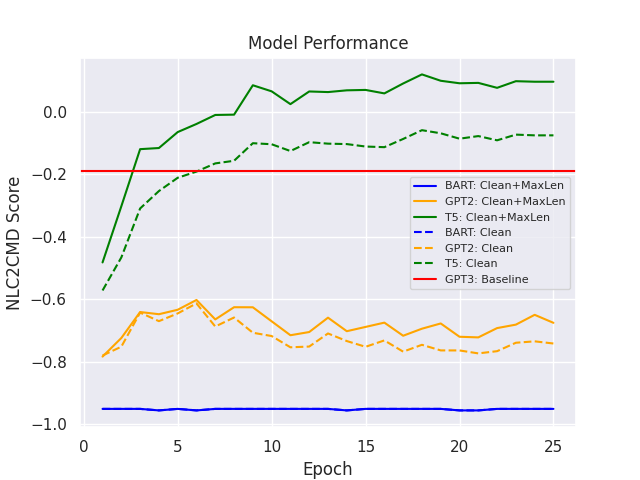
\includegraphics[scale=0.4]{metric.png}
\end{center}
The requirement from the course website: Report the quantitative results that you have found so far. Use a table or plot to compare results and compare against baselines.
Comment on your quantitative results. Are they what you expected? Better than you expected? Worse than you expected? Why do you think that is? What does that tell you about your approach?

Yingxiao's thought: show them the loss-epoch curve, the metric-epoch curve, and one table summarizing the best scores for the gpt2, bart, t5, and baseline gpt3, with different postprocessing functions. Please comment as much as you could in this section. Mention that our results became better and better after more epochs, although the score did not improve. Any thought on the causual / seq2seq models?


\section{Analysis}
One thing worth exploring is that for BART and GPT-2, although the training loss kept decreasing over epochs, the score was not improved that much. The raw model predictions have been extracted before postprocessing at the end of every epoch, and below is one example from the BART model:
\begin{verbatim}
invocation: display all the html files in the current folder excluding 
            search in the path ./foo,
target: find Path -path Regex -prune -or -type f -name Regex
\end{verbatim}
The prediction after the first epoch is
\begin{verbatim}
findfind Path -name Regex -prune -or -name f -name Regexexecexecexecexecexec
execexecexecexecexecexecexecexecexec
\end{verbatim}
the prediction after the sixth epoch is
\begin{verbatim}
Path -path Regex -prune -or -path f -name Regex -findfindfindfind
\end{verbatim}
and the prediction after the fourteenth epoch is
\begin{verbatim}
findfind Path -path Regex -prune -or -name f -name Regex -print - -
\end{verbatim}
Although none of the predictions correctly captured the target command, the model actually was learning something during training and pruned the trailing garbage itself at the end. However, the model still missed the flag "-type" and output many redundant ones (but not totally nonsense), not much improvement in score was made.

Also, one common error for all three models is unnecessary command sequences and here is one example
\begin{verbatim}
target    : cat File | sort -r -h 
prediction: cat File | sort -n -r | grep -v Regex
\end{verbatim}
Another type of error is the repeating sequences shown in the example below
\begin{verbatim}
target    : mount -o remount,ro -t yaffs2 Regex Regex 
prediction: mount Regex -o remount,rw Regex mount Regex -o remount,rw Regex 
            mount Regex -o remount, rw ...
\end{verbatim}
where the model didn't know when to stop. 

Such problems may be alleviated by using more robust models with defined penalty functions. Also, the number of examples we got is only 10,000, and a larger dataset will help to improve the model performance. 

\section{Conclusion}
Summarize the main findings of your project, and what you have learnt. Highlight your achievements, and note the primary limitations of your work. If you like, you can describe avenues for future work.


\bibliographystyle{unsrt}
\bibliography{references}


\appendix

\section{Appendix (optional)}
If you wish, you can include an appendix, which should be part of the main PDF, and does not count towards the 6-8 page limit.
Appendices can be useful to supply extra details, examples, figures, results, visualizations, etc., that you couldn't fit into the main paper. However, your grader \textit{does not} have to read your appendix, and you should assume that you will be graded based on the content of the main part of your paper only.

\end{document}
